Artificial Neural Networks (ANN's or short NN's) are a kind of data structure inspired by the biological neurons found in nature. They can be used to find a wide range of input output relations. One classic example is mapping pictures of hand written digits to the actual digits. Rather then explicitly program the relation NN's are trained on a dataset $(X, \, Y)$ of correct input output pairs.
\\


\begin{figure}[H]
    \centering
    \includegraphics[width=.6\linewidth]{bg_basic_nn}
    \caption{The most simple kind of NN is called densely connected or multilayer perceptron. For clarity only connections to the top most node of each layer are shown.}
    \label{fig:bg:basic_nn}
\end{figure}

\paragraph{Multilayer Perceptron}
This kind of classic NN consist of single nodes which are organized into layers. Every node is connected to all the nodes of the previous and next layer thus they are called dense. Each node holds a value called activation $a$ where the activation to the first layer is the input to the network, here:
$(x_1, \, x_2, \, x_3)$.
To calculate the activation of a node one has to multiply all the activations of the previous layer with their respective weights $w$, add the bias $b$ and finally apply a non-linear activation function $\sigma$. For the index notation superscripts specify the layer and subscripts the node. So $a^2_1$ is the activation of the first node in the second layer. To characterize a weight two subscripts are needed for the end and beginning of the connection. For the example in figure \ref{fig:bg:basic_nn} that means:

\begin{equation} \label{eq:bg:activation_example}
    a^2_1 = \sigma \qty(\sum_i w^2_{1i} \, x_i + b^2_1)
\end{equation}

\noindent
However it is more convenient to stop considering every node individually and to view the involved quantities as vectors and matrices. So that \eqref{eq:bg:activation_example} can be written as:

\begin{equation} \label{eq:bg:activation}
    \vb{a}^l = \sigma \qty(\vu{w}^l \vb{a}^{l-1} + \vb{b}^l)
\end{equation}

\begin{figure}[H]
\centering
\begin{subfigure}{.5\textwidth}
    \centering
    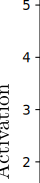
\includegraphics[width=\linewidth]{bg_relu}
    \caption{relu}
    \label{}
\end{subfigure}%
\begin{subfigure}{.5\textwidth}
    \centering
    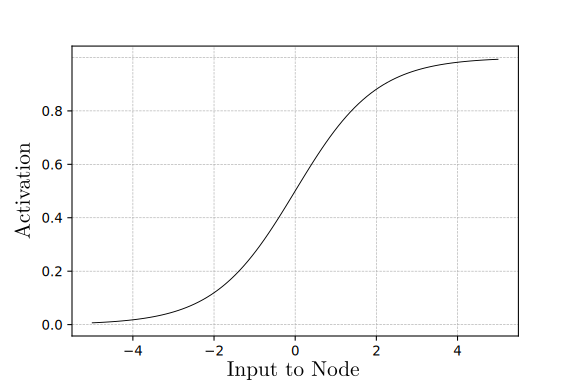
\includegraphics[width=\linewidth]{bg_sigmoid}
    \caption{sigmoid}
    \label{}
\end{subfigure}
\caption{Two examples of activation functions $\sigma$. Especially the relu function has a destinct on and off state similar to biological neurons.}
\label{}
\end{figure}

\paragraph{Training}
During training the network output $\s{NN}(\vb x) := \vb{y}' $ is calculated though repeated use of \eqref{eq:bg:activation} and is then compared with the known correct output $\vb y$ by a cost function $C = C(\vb y, \, \vb y')$. This might simply be the mean squared difference between $\vb y$ and $\vb y'$:

\begin{equation}
    C_\s{mse}(\vb y, \, \vb y') = \sum_i \qty(y_i - y_i')^2
\end{equation}

\noindent
but there are more sophisticated cost functions for different kind of outputs. Now we can quantify how well the NN is performing but how should the weights and biases be changed to improve this performance?
Here the very important Algorithm \textit{Backpropagation} is used and allows a efficient calculation of $\grad{C}_{\vb{b}^l}$ and $\grad{C}_{\vu{w}^l}$. These are used to gradually change the weights and biases to minimize the cost function. A very comprehensive explanation of Backpropagation can be found here: \cite{backprop}.

\paragraph{Convolutional Neural Networks}
An area where NNs have been very successful is image recognition or more general computer vision but the described multilayer perceptron has a number of weaknesses for this kind of task. Let's say our input is a $n$ by $n$, gray scale image. This can be expressed as a $n \cp n$ matrix, flattened and fed into the input layer (see figure \ref{fig:bg:flatten}). But now the number of weights to the next layer $\vu{w}^2$ are in the order of
$\order{n^3}$ (<- guess)
which soon becomes unfeasible.

\begin{figure}[H]
    \centering
    \includegraphics[width=.45\linewidth]{bg_flatten}
    \caption{Flattening of a $3\cp3$ matrix to fit the input of a multilayer perceptron.}
    \label{fig:bg:flatten}
\end{figure}

Computational limits aside there is another problem. Imagine an image with the letter T in the top right corner. If this letter moves to a different position the networks reaction will be completely different because the weights and biases involved are completely different. So the NN cannot learn the concept "letter T" independent of its position in the picture. Also the information about the distance between pixels is lost.

\begin{figure}[H]
    \centering
    \includegraphics[width=.6\linewidth]{bg_convnet_T}
    \caption{Two pictures of a T at different positions where the red color signifies a high value in the grayscale image. After the flatten operation seen in figure \ref{fig:bg:flatten} very different nodes are active.}
    \label{fig:bg:convnet_T}
\end{figure}

These problems led to the development of a new kind of layer called \textit{Convolution}. A fixed size \textit{kernel} is shifted over the matrix and at every position the the point wise product between kernel and matrix is calculated and summed. The result is called feature map of that kernel (see figure \ref{fig:bg:convolution}). Notice how the greatest value of the feature map is at the position of the letter T. So with only a small number of weights the convolution is able to detect the T independent of its position in the image. One convolutional layer contains not only a single but a number of different kernels $k$ so that the shape of the $n \times n$ matrix transforms to $(n-1) \times (n-1) \times k$. In a Convolutional Network (ConvNet) multiple of these layers are used so that it can find "patterns in patterns". For the letter detection example one could imagine the first layer to detect various edges and the next layer to detect letters in the position of these edges.

\begin{figure}[H]
    \centering
    \includegraphics[width=.6\linewidth]{bg_convolution}
    \caption{Example of a convolution where white pixel are 0 and red pixel are 1. The "T kernels" feature map is greatest at the position of the original letter.}
    \label{fig:bg:convolution}
\end{figure}

\paragraph{Pooling Layers}
For a big image and and a large number of kernels the output shape of a convolutional layers is still $n \times n \times k$, so quite large. Also notice how the "T kernel's" feature map is not only active at the exact position of the T but in the general region. The solution to this is to downsample the output with a \textit{Pooling Layer}. Here a smaller kernel, usually $2 \times 2$ is shifted over the matrix two steps at a time and at every position an operation is performed to reduce the number values to one. This could be taking the maximum or the average. This operation reduces the matrix in the x and y dimension by a factor of 2.

\begin{figure}[H]
    \centering
    \includegraphics[width=.6\linewidth]{bg_pooling}
    \caption{Example of a Max Pooling Layer. For every 2 by 2 field the maximum is calculated. After applying first the convolution and then the pooling layer the information "T in the top right corner" is still there and size of the resulting matrix is very manageable}
    \label{fig:bg:pooling}
\end{figure}

\paragraph{Example Network Architecture}
Now all the building blocks for a complete ConvNet are available. Repeatedly alternating convolution and pooling changes the input from wide in x and y dimension and narrow in z to a long z-strip. At the very end this strip is fed into one densely connected layer which is in turn connected to the output neurons.

\begin{figure}[H]
    \centering
    \includegraphics[width=.8\linewidth]{conv_net_example}
    \caption{Example for a complete ConvNet. Note the input is in this case an RGB image so there are three layers in the z dimension corresponding to the different colors. In this case the the first layer has 64 kernels of size $3 \times 3 \times 3$. The next convolution then has 128 kernels of size $3 \times 3 \times 64$. [citation needed]}
    \label{}
\end{figure}

\paragraph{1D ConvNets}
The algorithm is applied to spectra, so a functions $I(\lambda)$. This data is only one dimensional but all the same ideas apply. Kernels are here sized $1 \times 3 \times z$ and are shifted in one dimension. Same goes for the pooling. These 1D convolution might detect features like rising and falling edges.

\begin{figure}[H]
    \centering
    \includegraphics[width=.4\linewidth]{bg_1D_conv}
    \caption{Example of a 1D convolution. A $1 \times 3$ kernel is shifted over a spectrum $I$ discretized at 9 wavelengths}
    \label{fig:bg:1D_conv}
\end{figure}
